\section{Design Patterns}

Design patterns er guidelines for hvordan man kan designe programmer og klasser. De kan betragtes som generelle løsninger til generelle problemer. Konceptet begrænser sig ikke til datalogi, og blev faktisk opfundet af en arkitekt. Design patterns kan sammenlignes med algoritmer som også er software mønstre, men algoritmer løser beregningsproblemer, mens design patterns løser designproblemer.

\subsection{Observer Pattern}

\begin{itemize}
  \item Hvis et objekt (Subject) starter events (som fx “mine data har ændret sig”), som andre objekter (Observers) er interesserede i at vide noget om, kan man bruge OBSERVER mønstret. Stort set alle GUI elementer (fx knapper, checkboxes, slidere) er “Subjects” i implementationer som følger OBSERVER mønstret.
  \item Subject har en samling observer objekter, som bliver tilknyttet med en attach() metode. Når en event sker, meddeler subjectet det til alle observerne.
  \item Eksempel: JButtons (Subject) har ActionListeners (Observers). Ofte bruges anonyme klasser i stedet for at lave ConreteObserver klasser:
  \begin{verbatim}
    myButton.addActionListener(new ActionListener() { 
        public void actionPerformed(ActionEvent e) {
            // do something
        }
    });
  \end{verbatim}
  
  \begin{center}
    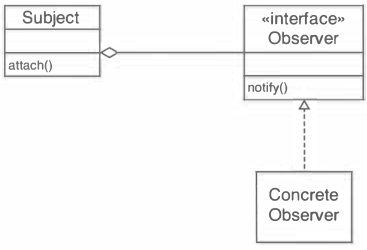
\includegraphics[scale=0.8]{images/observer_horstman.png}
  \end{center}

\end{itemize}




\subsection{Template Method Pattern}

\begin{itemize}
  \item Hvis en algoritme eller metode er brugbar i flere klasser, og kan brydes ned i “primitive operationer” (som godt kan være defineret forskelligt i de forskellige klasser) kan man bruge TEMPLATE METHOD mønstret.
  \item Metoden eller algoritmen, \verb|templateMethod()|, flyttes ind i en abstract superclass, sammen med abstract metoder for hver af de “primitive operationer”, som \verb|templateMethod()| kalder. Disse primitive operationer defineres IKKE i superclassen, men i subclasses (som extender den abstrakte superclass). 
  \item Altså er en \verb|templateMethod()| en metode som kalder andre metoder som ikke endnu er blevet defineret.
  \item Eksempel: \verb|drawSelection()| i SelectableShape - \verb|drawSelection()| er defineret i SelectableShape, men kalder metoder \verb|draw()| og \verb|translate()|, som er abstract methods i SelectableShape, men som bliver defineret i CarShape og HouseShape.
    
  \begin{center}
    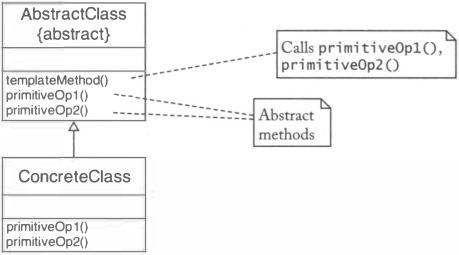
\includegraphics[scale=0.8]{images/template_method_horstman.png}
  \end{center}

\end{itemize}

\subsection{Strategy Pattern}

\begin{itemize}
  \item Hvis en klasse kan udnytte forskellige variationer af en algoritme, kan man bruge STRATEGY mønstret. LayoutManagers i Java er designet omkring STRATEGY mønstret. Containers (Context, fx JPanel, JFrame) kan udnytte forskellige layout managers (ConcreteStrategy, fx BorderLayout, GridLayout) til at arrangere deres indhold.
  \item De forskellige variationer af algoritmen defineres i klasser som implementerer et Strategy-interface. Context-klassen kalder så den rigtige metode på det konkrete Strategy-objekt. Dvs. enhver klasse som implementerer Strategy-interfacet kan benyttes af Context-klassen, men Context-klassen er også afhængig af (dependency) Strategy-interfacet.
  
  \begin{center}
    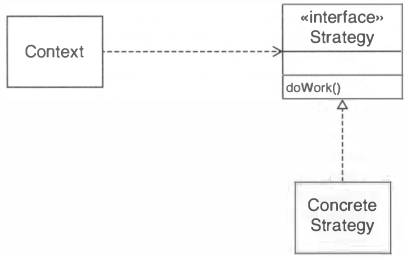
\includegraphics[scale=0.7]{images/strategy_horstman.png}
  \end{center}

\end{itemize}

\subsection{Composite Pattern}

\begin{itemize}
  \item Hvis man har behov for at kombinere en række primitive objekter i en “bundle”, som bliver opfattet af klienter som værende et enkelt primitivt objekt selv, kan man benytte COMPOSITE mønstret.
  \item Man lader en klasse (Composite) implementere det samme interface som det, de primitive objekter implementerer. Composite-klassen betragtes således af klienter på samme måde som de primitive objekter. Desuden aggregerer Composite-klassen også interfacet, hvilket betyder at den har en samling (fx ArrayList) af primitive objekter.
  \item Metoderne fra interfacet defineres i Composite-klassen ved at kalde metoderne på hvert af de primitive objekter, som er indeholdt i klassen. De skal selvfølgelig kaldes på en bestemt måde - fx skal en Bundle-klasse som indeholder Item-objekter udregne alle Item-objekternes samlede pris, når \verb|getPrice()| kaldes på Bundle.
  
  \begin{center}
    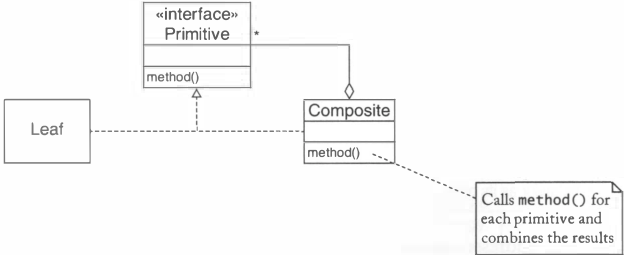
\includegraphics[scale=0.8]{images/composite_horstman.png}
  \end{center}

\end{itemize}

